%-------------------------------------------------------------------------------
% seq24_menu
%-------------------------------------------------------------------------------
%
% \file        seq24_menu.tex
% \library     Documents
% \author      Chris Ahlstrom
% \date        2015-07-19
% \update      2016-05-20
% \version     $Revision$
% \license     $XPC_GPL_LICENSE$
%
%     Provides the Menu section of seq24-user-manual.tex.
%
%-------------------------------------------------------------------------------

\section{Menu}
\label{sec:seq24_menu}

   The \textsl{Seq24} menu, as seen at the top of
   \figureref{fig:seq24_main_screen}, is fairly simple, but it is important to
   understand the structure of the menu entries.

\subsection{Menu / File}
\label{subsec:seq24_menu_file}

   The \textbf{File} menu is used to save and load standard MIDI files.
   \textsl{Seq24} should be able to handle any Format 1 standard files that any
   other sequencer is capable of exporting.  

   The \textsl{Seq24} menu entry contains the sub-items shown in
   \figureref{fig:seq24_menu_file_items}.  The next few sub-sections discuss the
   sub-items in the \textsl{File} sub-menu.

\begin{figure}[H]
   \centering 
   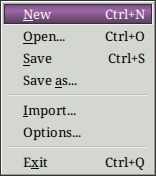
\includegraphics[scale=0.75]{menu/menu_file.png}
   \caption{Seq24 File Menu Items}
   \label{fig:seq24_menu_file_items}
\end{figure}

   \begin{enumber}
      \item \textbf{New}
      \item \textbf{Open...}
      \item \textbf{Save}
      \item \textbf{Save As...}
      \item \textbf{Import...}
      \item \textbf{Options...}
      \item \textbf{Exit}
   \end{enumber}

\subsection{Menu / File / New}
\label{subsec:menu_file_new}

   The \textbf{New} menu entry clears out any current song and patterns,
   allowing one to create news ones from scratch.
   If unsaved changes are pending, the user will be prompted to save the
   changes.

\subsubsection{Menu / File / Open}
\label{subsubsec:seq24_menu_file_open}

   The \textbf{Open} menu entry opens a song that had been saved previously.
   It opens up a standard GTK+2 file dialog.

\begin{figure}[H]
   \centering 
   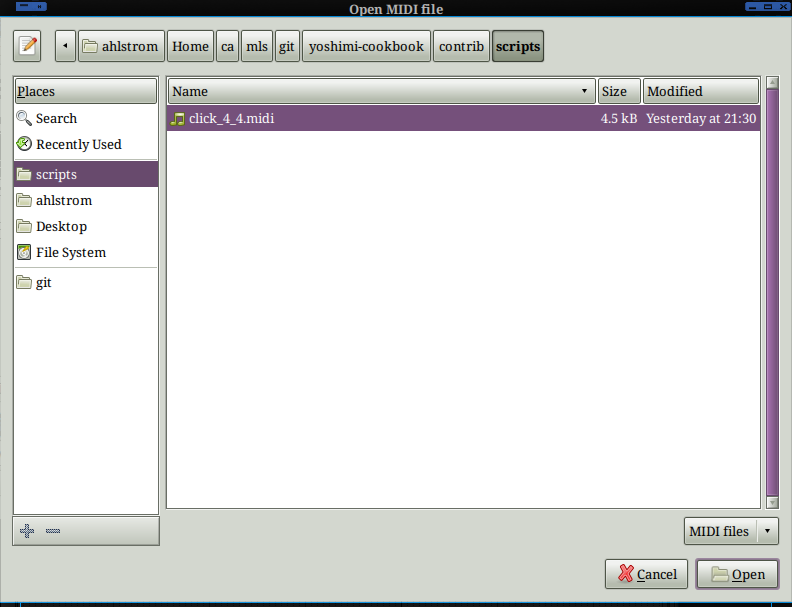
\includegraphics[scale=0.65]{menu/menu_file_open.png}
   \caption{File Open}
   \label{fig:seq24_menu_file_open}
\end{figure}

   If unsaved changes are pending, the user will be prompted to save the
   changes.  When in doubt, save!  If still in doubt, keep backups of your
   tunes!

\subsubsection{Menu / File / Save and Save As}
\label{subsubsec:menu_file_open_save_as}

   The \textbf{Save} menu entry saves the song under its current name.
   If there is no current name, then
   it opens up a standard GTK+2 file dialog.

   The \textbf{Save As} menu entry saves a song under a different name.
   It opens up the following standard GTK+ file dialog.

\begin{figure}[H]
   \centering 
   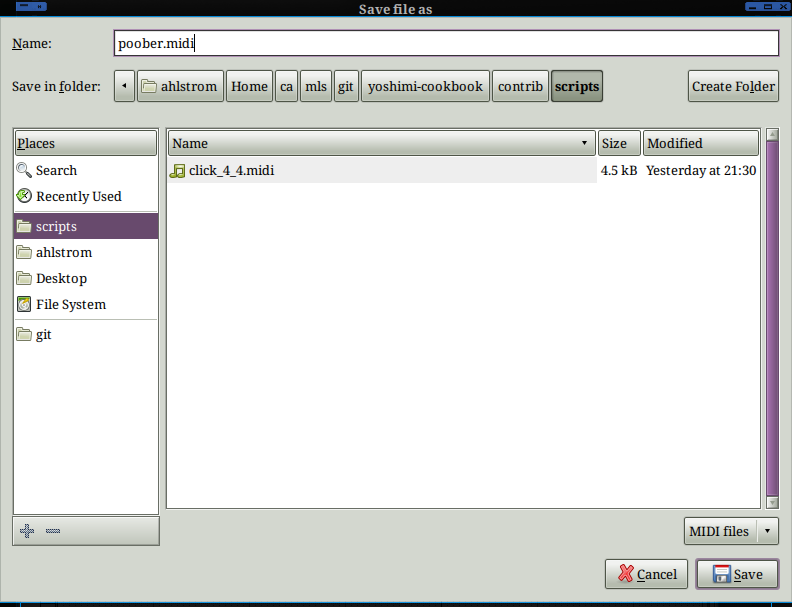
\includegraphics[scale=0.65]{menu/menu_file_save_as.png}
   \caption{File Save As}
   \label{fig:seq24_menu_file_save_as}
\end{figure}

   To save a new file, or to save the current existing file to a new name,
   enter the name in the name field, \textsl{without an extension}.
   \textsl{Seq24} will append a \texttt{.midi} extension to the filename.

   The file will be save in a format the the Linux \textsl{file} command
   will tag as something like:

   \begin{verbatim}
      myfile.midi: Standard MIDI data (format 1) using 16 tracks at 1/192
   \end{verbatim}

   \index{todo!solve seq24 format}
   It looks like a simple MIDI file, and yet, if one re-opens it in
   \textsl{Seq24}, one sees that all of the labelling, pattern information,
   and song layout has been preserved in this file.
   Even the pattern subsections, as discussed in
   \sectionref{subsubsec:seq24_song_editor_arrangement_panel_roll},
   have been saved.
   (But the L and R marker positions are not saved.)

   Compare the sizes of the original project MIDI file,
   \texttt{contrib/b4uacuse.mid}, and the output MIDI file after
   \textsl{Seq24} saved the patterns and the song layout we created,
   \texttt{contrib/b4uacuse-seq24.midi}.  The latter is a lot
   bigger.  

\subsubsection{Menu / File / Import}
\label{subsubsec:seq24_menu_file_import}

   The \textbf{Import} menu entry allows one to import a MIDI file
   into a pattern.

\begin{figure}[H]
   \centering 
   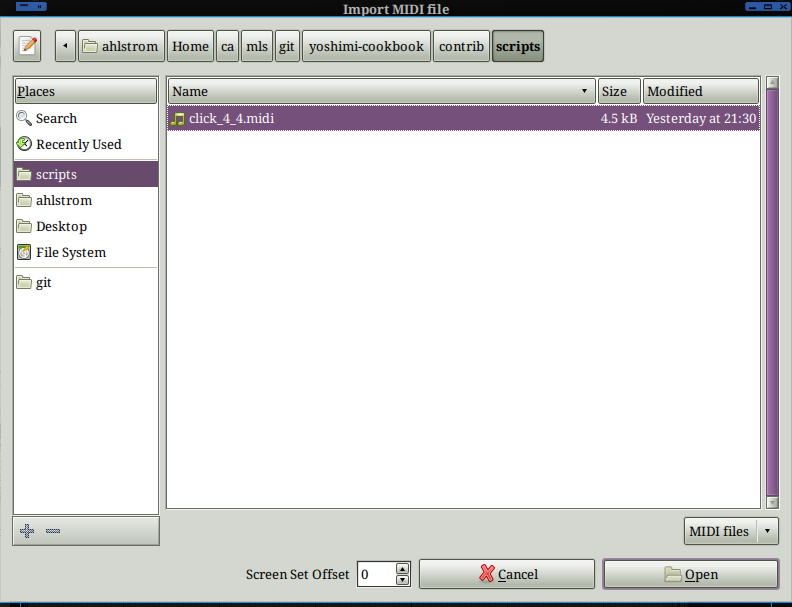
\includegraphics[scale=0.65]{menu/menu_file_import.png}
   \caption{File Import}
   \label{fig:seq24_menu_file_import}
\end{figure}

   When imported, each track, whether a music track or an information track,
   is entered into its own loop/pattern box.  The import operation can
   handle reasonably complex files, as shown in the following diagram, which
   shows an import of the \texttt{contrib/b4uacuse.mid} file, which contains
   a transcription of an Eric Clapton tune that we'd made over 20 
   years ago and had uploaded to the \textsl{GEnie} network service.

   Note the additional file-dialog field,
   \textbf{Select Screen Offset}.
   \index{import!select screen offset}
   \index{select screen offset}
   This setting lets one place the imported data into a screen-set other than
   the first screen-set, screen-set 0.
   This field is not editable.  It requires using the scroll button to move the
   screen set offset up or down in value.  The legal values range from -31 to 0
   to +31.
   
   When the file is imported, the sequence number for each track read in is
   adjusted to put the track in the desired screen set.  The negative numbers
   are probably more useful to move sequences around in an already-created
   \textsl{Seq24} song file with a lot of screen-sets in it.

\begin{figure}[H]
   \centering 
   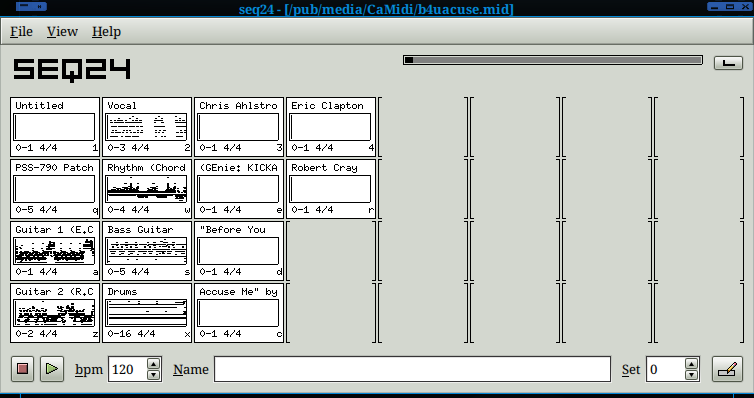
\includegraphics[scale=0.90]{menu/imported_midi_song.png}
   \caption{Imported MIDI Song}
   \label{fig:seq24_imported_midi_song}
\end{figure}

   Unfortunately, this song was created before the days of General MIDI.
   It is scored for the Yamaha PSS-790 consumer-level synthesizer.
   One can use our MIDI-conversion project (see reference \cite{midicvt}) 
   to convert it to General MIDI format, including General MIDI drums.

\subsubsection{Menu / File / Options}
\label{subsubsec:seq24_menu_file_options}

   The \textbf{Options} menu item provides a number of settings in one
   tabbed dialog, shown in the figure below.
   This dialog allows one to select which sequence gets the MIDI
   clock, which incoming MIDI events control the sequencer, what keys are
   mapped to functions, how the mouse works, and some JACK parameters.

\paragraph{Menu / File / Options / MIDI Clock}
\label{paragraph:seq24_menu_file_options_midi_clock}

   The \textbf{MIDI Clock} tab provides a way to send the MIDI clock to one
   or more of the \textsl{Seq24} output busses.
   It is used to configure to what busses the MIDI clock gets dumped.
   It also shows the devices that one can play music with.
   The items that appear in this tab depend on three things:

   \begin{itemize}
      \item What MIDI devices are connected to the computer.  For example,
         MIDI controllers, USB MIDI cables, and other devices will add MIDI
         output devices (ports) to the system.
      \item What MIDI software devices are running on the computer.
         For example, running MIDI software synthesizers such as
         \textsl{Timidity} and \textsl{Yoshimi} will add extra output devices
         (playback ports) to a system.
      \item The setting of the "manual ALSA ports" option,
         \texttt{--manual\_alsa\_ports} command-line option or the
         \texttt{[manual-alsa-ports]} section of the
         \texttt{seq24rc} configuration file.
   \end{itemize}

   For the current discussion, a USB MIDI cable was plugged into the system,
   and the \textsl{Timidity} and \textsl{Yoshimi} (in ALSA mode) software
   synthesizers were running.  \textsl{Seq24} was also running, of
   course.  Here are the devices shown by the ALSA MIDI playback
   command-line application:

   \begin{verbatim}
      $ aplaymidi -l
       Port    Client name                      Port name
       14:0    Midi Through                     Midi Through Port-0
       24:0    USB2.0-MIDI                      USB2.0-MIDI MIDI 1
       24:1    USB2.0-MIDI                      USB2.0-MIDI MIDI 2
      128:0    TiMidity                         TiMidity port 0
      128:1    TiMidity                         TiMidity port 1
      128:2    TiMidity                         TiMidity port 2
      128:3    TiMidity                         TiMidity port 3
      130:16   seq24                            seq24 in
   \end{verbatim}

   (For some reason, the \textsl{Yoshimi} input port is not showing up
   in the output of \texttt{aplaymidi}.
   \textsl{Seq24} sees it on port 7.  Perhaps that application is not
   providing a good ALSA device name.)
   

\begin{figure}[H]
   \centering 
   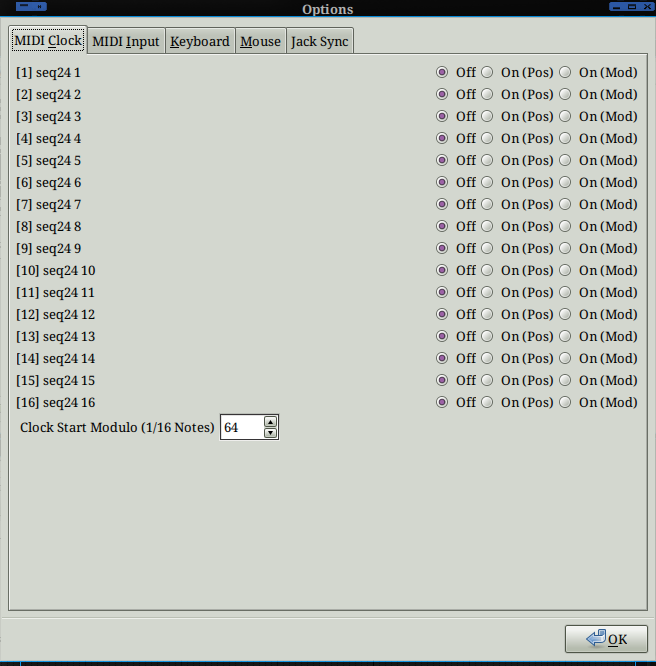
\includegraphics[scale=0.75]{menu/menu_file_options_midi_clock.png}
   \caption{File / Options / MIDI Clock}
   \label{fig:seq24_menu_file_options_midi_clock}
\end{figure}

   The following elements are present in this dialog:

   \begin{enumber}
      \item \textbf{Buss Name}
      \item \textbf{Off}
      \item \textbf{On (Pos)}
      \item \textbf{On (Mod)}
      \item \textbf{Clock Start Modulo}
   \end{enumber}

   \setcounter{ItemCounter}{0}      % Reset the ItemCounter for this list.

   \itempar{Buss Name}{midi clock!buss name}
   These labels indicate the output busses of \textsl{Seq24}.
   They range from \textbf{[1] seq24 1}
   to \textbf{[16] seq24 16}.

   \itempar{Off}{midi clock!off}
   This setting disables the MIDI clock for the given output buss.
   However, note that MIDI output can still be sent to those ports, and
   each port that has a device connected to it will play music.
   
   For feeding \textsl{Yoshimi} with MIDI data, we found that this
   setting is the one that must be made in order for \textsl{Yoshimi} to
   produce a sound.

   \itempar{On (Pos)}{midi clock!on (pos)}
   The MIDI clock will be sent to this buss.
   MIDI Song Position and MIDI Continue will be sent if playback is starting
   at greater than tick 0 in Song mode.  Otherwise, MIDI Start will be sent.

   \itempar{On (Mod)}{midi clock!on (mod)}
   The MIDI clock will be sent to this buss.
   MIDI Start will be sent and clocking will begin
   once the Song Position has reached the start modulo of the specified size
   (see the next item's description).
   This setting is used for gear that does not respond to Song Position.

   \itempar{Clock Start Modulo}{midi clock!clock start modulo}
   Clock Start Modulo (1/16 Notes).
   This value starts at 1 and ranges on upward to 16384.
   It  defaults to 64.
   It is used by the \textbf{On (Mod)} setting discussed above.
   It is the \texttt{[midi-clock-mod-ticks]} option in the \textsl{Seq24}
   "rc" file as described in
   \sectionref{subsec:seq24_rc_file_other_midi}.

   With the manual ALSA option turned off,
   all of the devices that can be driven by MIDI output are shown,
   including the MIDI Thru port, the two MIDI ports on the USB cable,
   the four ports provided by \textsl{Timidity}, and the unlabelled
   port provided by \textsl{Yoshimi}.

   One could theoretically play music through 6 or 7 devices using
   \textsl{Seq24} with this setup.

\paragraph{Menu / File / Options / MIDI Input}
\label{paragraph:seq24_menu_file_options_midi_input}

   To allow \textsl{Seq24} to record MIDI from MIDI devices such as
   controllers and keyboards, the output of the ALSA MIDI recording
   command-line application is relevant:

   \begin{verbatim}
      $ arecordmidi -l
       Port    Client name                      Port name
       14:0    Midi Through                     Midi Through Port-0
       24:0    USB2.0-MIDI                      USB2.0-MIDI MIDI 1
      130:0    seq24                            [1] seq24 1
      130:1    seq24                            [2] seq24 2
      130:2    seq24                            [3] seq24 3
       . . .   . . .                               . . .
      130:15   seq24                            [16] seq24 16
   \end{verbatim}

   The only item in the \textbf{MIDI Input} tab is the single MIDI input
   buss provided by \textsl{Seq24}:  \textbf{[0] seq24 0}.

   If the "manual ALSA ports" option (see below) is turned on,
   then the only item in the \textbf{MIDI Input} tab is the single MIDI input
   buss provided by \textsl{Seq24}:  \textbf{[0] seq24 0}, or, since
   the MIDI Thru port takes slot 0, \textbf{[1] seq24 1}.

\begin{figure}[H]
   \centering 
   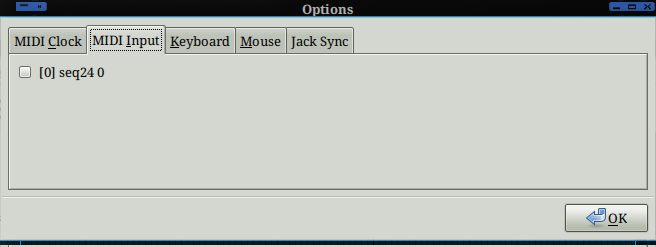
\includegraphics[scale=0.75]{menu/menu_file_options_midi_input_condensed.png}
   \caption{File / Options / MIDI Input (Condensed View)}
   \label{fig:seq24_menu_file_options_midi_input}
\end{figure}

   This item, if checked allows \textsl{Seq24} to be used to record MIDI
   information from another source, or pass it through to the output busses
   that are configured
   to allow pass-through
   (in the Pattern Editor, as discussed in 
   \sectionref{subsec:seq24_pattern_editor_bottom}.)

   If the "manual ALSA ports" option is turned off, then
   the input ports from the system are shown.
   For example, one could check input \#1 to have \textsl{Seq24} record
   MIDI from an old-fashioned MIDI keyboard that is connected to the USB MIDI
   cable.  If the keyboard didn't have a sound generator, one would also want
   \textsl{Seq24} to pass this MIDI on to a sound generator, such as a
   software or hardware synthesizer attached to one of the ports.

\paragraph{Menu / File / Options / Keyboard }
\label{paragraph:seq24_menu_file_options_keyboard}

   \textsl{Seq24}, as befits a good application, allows extensive use of
   keyboard shortcuts to make operations go faster than when using a mouse.
   The \textbf{Keyboard} tab allows for the configuration of these keyboard
   shortcuts.

\begin{figure}[H]
   \centering 
   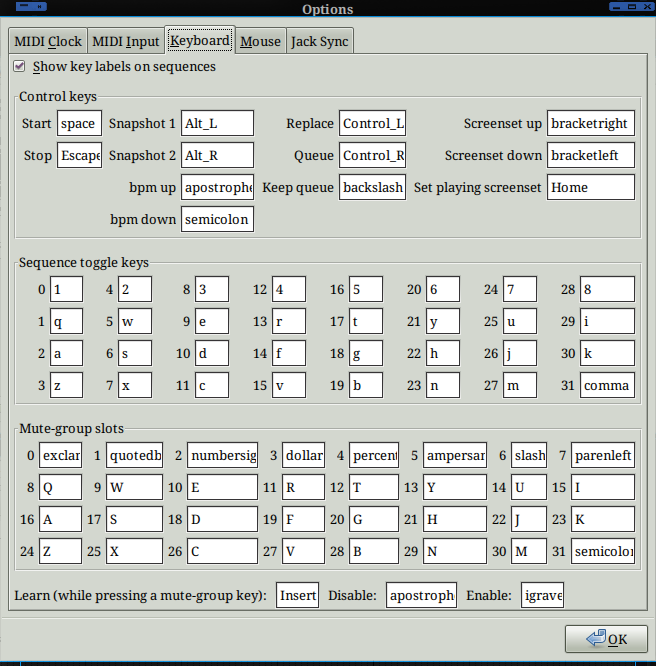
\includegraphics[scale=0.75]{menu/menu_file_options_keyboard.png}
   \caption{File / Options / Keyboard}
   \label{fig:seq24_menu_file_options_keyboard}
\end{figure}

   We won't attempt to cover every user-interface item in this busy
   dialog, just the categories.

   \begin{enumber}
      \item \textbf{Show key labels on sequences}
      \item \textbf{Control keys}
      \item \textbf{Sequence toggle keys}
      \item \textbf{Mute-group slots}
      \item \textbf{Learn}
      \item \textbf{Disable}
      \item \textbf{Enable}
   \end{enumber}

   \setcounter{ItemCounter}{0}      % Reset the ItemCounter for this list.

   \itempar{Show key labels on sequence}{keyboard!show labels}
   This item, if enabled, shows the key labels in the lower-right corner of
   each loop/pattern in the Patterns window.

   \itempar{Control keys}{keyboard!control keys}
   This block of fields provides shortcut keys for many operations of
   \textsl{Seq24}.

   \begin{enumber}
      \item \textbf{Start}.
         Key: \index{keys!space} \textbf{space}.
      \item \textbf{Stop}.
         Key: \index{keys!esc} \textbf{Escape}.
      \item \textbf{Snapshot 1}.
         Key: \index{keys!alt-l} \textbf{Alt\_L}.
      \item \textbf{Snapshot 2}.
         Key: \index{keys!alt-r} \textbf{Alt\_R}.
      \item \textbf{bpm up}.
         Key: \index{keys!apostrophe} \textbf{apostrophe}.
      \item \textbf{bpm down}.
         Key: \index{keys!semicolon} \textbf{semicolon}.
      \item \textbf{Replace}.
         Key: \index{keys!ctrl-l} \textbf{Control\_L}.
      \item \textbf{Queue}.
         Key: \index{keys!ctrl-r} \textbf{Control\_R}.
      \item \textbf{Keep queue}.
         Key: \index{keys!backslash} \textbf{backslash}.
      \item \textbf{Screenset down}.
         Key: \index{keys![} \textbf{bracketleft}.
      \item \textbf{Screenset up}.
         Key: \index{keys!]} \textbf{bracketright}.
      \item \textbf{Set playing screenset}.
         Key: \index{keys!home} \textbf{Home}.
   \end{enumber}

   Note that some of the keys have positional mnemonic value.  For example,
   for BPM control, the semicolon is at the left (down), and the apostrophe
   is at the right (up).

   Also note that the keys definable in this tab are only a subset of the
   various keys that can be used, especially keys used with the
   \texttt{Ctrl} key.

   TODO:  \index{todo!snapshot definition}
   One thing we need to figure out is just what this "snapshot"
   feature provides.
   \index{todo!keep queue}
   Another thing is the "queue" and "keep queue" features.

   \index{queue}
   To "queue" a pattern means to ready it for playback upon the next repeat
   of a pattern.  A pattern can be armed immediately, or it can be queued to
   play back the next time the pattern starts.
   A pattern can be queued by holding the queue key (defined in
   \textbf{File / Options / Keyboard / queue}) and pressing a pattern-slot
   shortcut key.  Instead of the pattern turning on immediately, it turns on at
   the next repeat of the pattern.

   \index{keep queue}
   \index{queue!keep}
   The "keep queue" functionality allows the queue to be held without holding
   down the queue button the whole time.  First, press the keep-queue key
   (defined in \textbf{File / Options / Keyboard / Keep queue}).  Now, hitting
   any of the shortcut keys, no matter how many, sets up the corresponding
   pattern slot to be queued.  This mode is disabled by hitting the
   "queue" key (any currently active queues remain active until finished).

   \itempar{Sequence toggle keys}{keyboard!sequence toggle keys}
   Each of these keys toggles the playing/muting of one of the 32
   loop/pattern boxes.  These keys are layed out logically on the keyboard,
   and can also be shown in each loop/pattern box.  No need to list them all
   here!

   \itempar{Mute-group slots}{keyboard!mute-group slots}
   Each of these keys operates on the mute-grouping of one of the 32
   loop/pattern boxes.  These keys are layed out logically on the keyboard,
   and can also be shown in each loop/pattern box.  No need to list them all
   here!

   \index{todo!mute-group}
   One thing we need to discover is just what this mute-grouping
   means functionally.
   Apparently groups work with the playing screen set only.
   Change the screenset and give the command to make it the playing one
   (e.g. set the HOME key for this purpose.)

   \itempar{Learn}{keyboard!learn}
   Learn (while pressing a mute-group key).
   This items sets the key used to initiate a learn mode.
   It is the \textbf{Insert} key by default.

   \itempar{Disable}{keyboard!disable}
   TODO: \index{todo!keyboard disable} What gets disabled?
   \index{keys!apostrophe}
   It is the \textbf{apostrophe} key by default.

   \itempar{Enable}{keyboard!enable}
   TODO: What gets enabled?
   \index{keys!igrave}
   It is the \textbf{igrave} (back-tick) key by default.

   There is much to learn about this learn/enable/disable triad!

\paragraph{Menu / File / Options / Mouse }
\label{paragraph:seq24_menu_file_options_mouse}

   This item selects the mouse-interaction method.

\begin{figure}[H]
   \centering 
   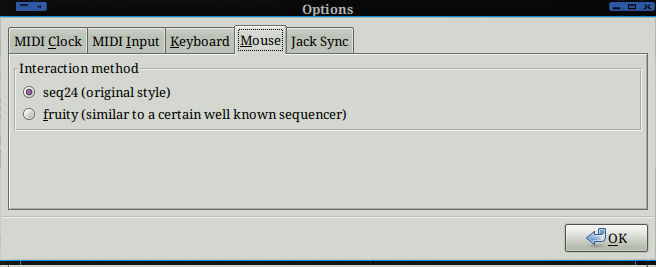
\includegraphics[scale=0.75]{menu/menu_file_options_mouse_condensed.png}
   \caption{File / Options / Mouse (Condensed View)}
   \label{fig:seq24_menu_file_options_mouse}
\end{figure}

   The default method is \textbf{seq24 (original style)}.
   The alternate method is \textbf{fruity (similar to a certain well known
   sequencer)}.

   \index{mouse!fruity}
   The alternate method is presumably that of the \textsl{Fruity Loops}
   (now \textsl{FL Studio}) sequencer.  The fruity mode seems to involve the
   following (based on scanning the source code):
   
   \begin{itemize}
      \item \textbf{Left-click left side}.
         Begin a grow/shrink operation for the left side.
      \item \textbf{Left-click right side}.
         Begin a grow/shrink operation for the right side.
      \item \textbf{Left-click middle}.
         Move the object.
      \item \textbf{Left-click}.
         Add an event if nothing selected.
      \item \textbf{Middle-click}.
         Split the note?
   \end{itemize}

   The \textsl{Seq24} "original style" is pretty much as expected for basic
   actions such as selecting and moving notes using the left mouse button.
   Drawing a note or event is a bit different, in the one must first
   \textsl{click and hold} the right mouse button, and then
   \textsl{click and drag} the right mouse button to insert notes,
   Notes are inserted to be at the current length and grid-snap values for
   the sequence editor for as long as the left button is pressed.
   Notes are inserted only up to the boundary of the sequence length.
   And, once notes are inserted, moving the mouse with the left button still
   held down simply moves the notes to the new note value of the mouse.

   If one releases the left button, then presses and holds it again,
   more notes will be added in the same way.
   This is strange, but it is a powerful way to layer notes into a short
   sequence.
   We call it the \index{draw mode} \index{mode!draw } "draw mode" or
   \index{paint mode} \index{mode!paint } "paint mode".

   Note that drawing/painting can also be done while the sequence is playing,
   and notes will be added to be played the next time the progress bar crosses
   them.

\paragraph{Menu / File / Options / Jack Sync }
\label{paragraph:seq24_menu_file_options_jack_sync}

   This tab sets up options for JACK synchronization.

\begin{figure}[H]
   \centering 
   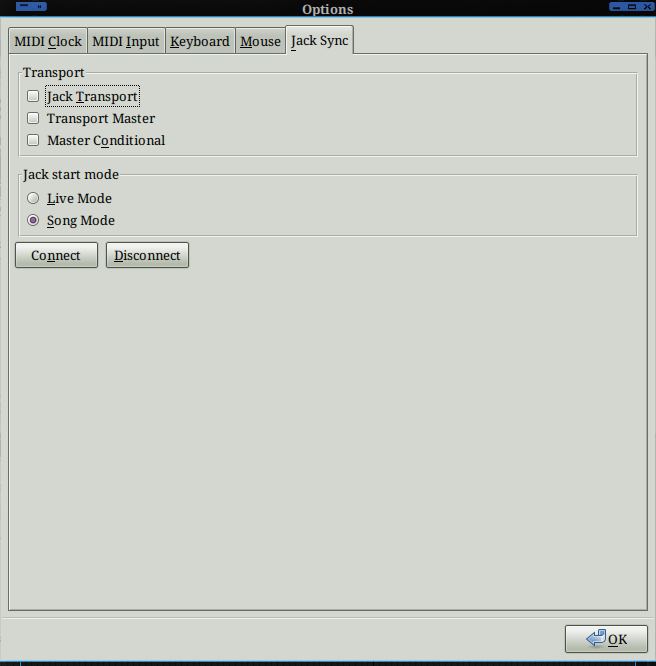
\includegraphics[scale=0.75]{menu/menu_file_options_jack_sync.png}
   \caption{File / Options / Jack Sync}
   \label{fig:seq24_menu_file_options_jack_sync}
\end{figure}

   \begin{enumber}
      \item \textbf{Transport}
      \item \textbf{Jack start mode}
      \item \textbf{Connect}
      \item \textbf{Disconnect}
   \end{enumber}

   \setcounter{ItemCounter}{0}      % Reset the ItemCounter for this list.

   \itempar{Transport}{jack sync!transport}
   These settings are stored in the "rc" file settings group
   \texttt{[jack-transport]}.
   This items collects the following settings:

   \begin{itemize}
      \item \textbf{Jack Transport}.
         \index{JACK!transport}
         Enables synchronization with JACK Transport.
      \item \textbf{Transport Master}.
         \index{JACK!transport master}
         \textsl{Seq24} will attempt to serve as the JACK Master.
      \item \textbf{Master Conditional}.
         \index{JACK!master conditional}
         \textsl{Seq24} will fail to serve as the JACK Master if there is
         already a Master set.
   \end{itemize}

   Note that there are long-standing issues with the JACK support of
   \textsl{Seq24}, and \textsl{Seq24} currently inherits some of them,
   in spite of some bug fixes.  Generally, if one experiences issues in
   transport control, try making one of the other sequencer applications the
   JACK Master.

   If one makes a change in the JACK settings, it is best to
   then press the \textbf{Disconnect} button, then the \textbf{Connect}
   button.  Another option is to restart \textsl{Seq24}... the settings
   are automatically saved when \textsl{Seq24} exits.

   \itempar{Transport}{jack sync!transport}
   This items collects the following settings:

   \begin{itemize}
      \item \textbf{Live Mode}.
         \index{JACK!live mode}
         \index{live mode}
         \index{non-playback mode}
         Playback will be in live mode.  Use this option to allow muting and
         unmuting of patterns.
         The command-line option is \texttt{--jack\_start\_mode 0}.
      \item \textbf{Song Mode}.
         \index{JACK!song mode}
         \index{song mode}
         \index{playback mode}
         \index{performance mode}
         Playback will use only the Song Editor's data.
         The command-line option is \texttt{--jack\_start\_mode 1}.
   \end{itemize}

   Note that, in ALSA mode (non-JACK mode), \textsl{Seq24} 
   now \textsl{does} select the playback modes
   according to which window started the playback.
   
   \textsl{The main window, or pattern
   window, causes playback to be in live mode.  The user can arm and mute
   patterns in that windows, by clicking on sequences, using their hot-keys,
   and by using the group-mode and learn-mode features (we think).
   The song editor causes playback to be in performance mode, also known as
   "playback mode", or "song mode".}

   Of course, in JACK mode,
   it selects them according to the chosen live/song mode as discussed above.
   \itempar{Connect}{jack sync!connect}
   Connect to JACK Sync.

   \itempar{Disconnect}{jack sync!disconnect}
   Disconnect from JACK Sync.

\subsection{Menu / View}
\label{subsec:seq24_menu_view}

   This menu item has only one entry, \textbf{Song Editor}, 
   which is already covered by a button at the bottom of the Patterns
   window.  Selecting this item bring up the Song Editor window.
   See \figureref{fig:song_editor_window}

   The Song Editor window can also be brought up via the
   \index{song editor!ctrl-e}
   \index{keys!ctrl-e}
   Ctrl-E key.
\subsection{Menu / Help About...}
\label{subsec:seq24_menu_about}

   This menu entry shows the "About" dialog.

\begin{figure}[H]
   \centering 
   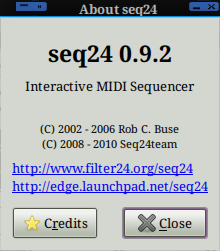
\includegraphics[scale=0.75]{menu/menu_help_about.png}
   \caption{Help About}
   \label{fig:seq24_menu_help_about}
\end{figure}

   That dialog provides access to the credits for the program, including the
   authors and the project documentor.

\begin{figure}[H]
   \centering 
   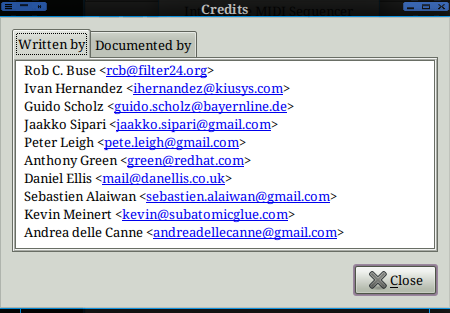
\includegraphics[scale=0.75]{menu/menu_help_credits.png}
   \caption{Help Credits}
   \label{fig:seq24_menu_help_credits}
\end{figure}

   Shows who has worked on the program, with the original author at the top
   of the list.

\begin{figure}[H]
   \centering 
   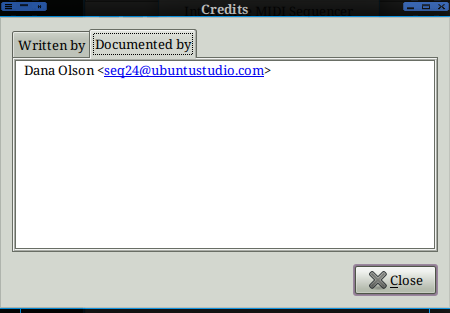
\includegraphics[scale=0.75]{menu/menu_help_doc.png}
   \caption{Help Documentation}
   \label{fig:seq24_menu_help_doc}
\end{figure}

   Shows who has documented this project.

%-------------------------------------------------------------------------------
% vim: ts=3 sw=3 et ft=tex
%-------------------------------------------------------------------------------
